% ============================================================
\chapter{Methods and Materials}
\label{ch:methods}
% ============================================================

This chapter describes the full experimental methodology, covering the dataset and its preprocessing, spatial clustering, feature engineering, and the ride pooling algorithm.  \autoref{fig:pipeline} illustrates the complete processing pipeline.

\begin{figure}[t]
  \centering
  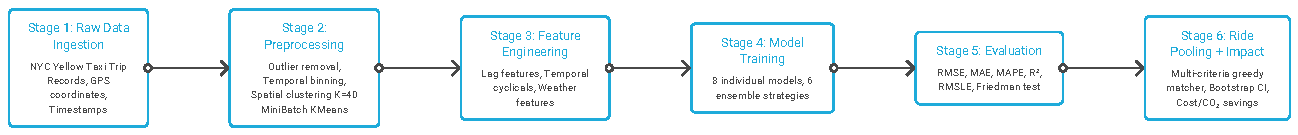
\includegraphics[width=\textwidth, height=0.52\textheight, keepaspectratio]{Figures/complete_pipeline.pdf}
  \caption{Complete research pipeline from raw data to city-scale impact: data ingestion, outlier removal, spatial clustering, temporal binning, feature engineering, model training and evaluation, ride pooling matching, bootstrap validation, and economic and CO\textsubscript{2} impact projection.}
  \label{fig:pipeline}
\end{figure}

\autoref{fig:pipeline} traces the end-to-end data flow through six sequential stages.  Stage~1 ingests the raw NYC Yellow Taxi Trip Records and applies coordinate boundary filtering, duration filtering, and fare filtering to remove implausible records.  Stage~2 constructs spatial zones via MiniBatch KMeans on a stratified 5\% sample of pickup coordinates, choosing $K{=}40$ as the cluster count validated by inertia elbow, silhouette score, and downstream prediction RMSE criteria.  Stage~3 aggregates trips into 10-minute bins per cluster and engineers the full feature set described in \autoref{tab:features}.  Stage~4 trains all 14 models under a strictly chronological 80/20 split and evaluates them across five metrics.  Stage~5 applies the multi-criteria ride pooling algorithm to a 106,055-trip sample, computing compatibility scores and greedy matches within 5-minute windows.  Stage~6 applies bootstrap resampling over 10,000 iterations to produce 95\% confidence intervals for pool rate, savings, and compatibility metrics, and scales the sample estimates to full NYC annual volume for city-wide impact projection.  Each stage is implemented as a modular Python notebook, facilitating independent validation and extension.


\section{Dataset}

This study uses the publicly available NYC Yellow Taxi Trip Records~\parencite{taxinyc_dataset} hosted on Kaggle.  The training split covers January 2015, comprising approximately 12.7 million trips, and the test split covers January to March 2016, comprising approximately 34 million trips.  Each record includes pickup and drop-off timestamps, GPS coordinates, passenger count, trip distance, and fare information.  \autoref{tab:dataset} summarises the dataset.

\begin{table}[t]
\centering
\caption{NYC Yellow Taxi dataset statistics.\label{tab:dataset}}
\begin{tabularx}{\textwidth}{>{\raggedright\arraybackslash}X r}
\toprule
\textbf{Attribute} & \textbf{Value} \\
\midrule
Training period & January 2015 \\
Testing period  & January--March 2016 \\
Approximate training trips & 12.7 million \\
Approximate test trips & 34 million \\
Spatial bounding box (lat) & 40.58 -- 40.92 \\
Spatial bounding box (lon) & $-$74.15 -- $-$73.70 \\
Features per record & 19 \\
\bottomrule
\end{tabularx}
\end{table}

\subsection{Chronological Train-Test Split}
A key methodological requirement for time-series data is that the training set precedes the test set in calendar time.  The split is \emph{strictly chronological}: the training set is drawn entirely from January 2015 and the test set from January--March 2016, separated by an 11-month gap.  At the aggregated feature-matrix level, records are sorted ascending by \texttt{datetime\_bin} and split at 80\% using \texttt{train\_test\_split(shuffle=False)}, ensuring no lag-feature from the future leaks into training.

The 11-month gap between training and test periods is a deliberate design choice rather than an artefact of data availability.  A contiguous split -- for example, training on January through October 2015 and testing on November through December 2015 -- would evaluate models on demand patterns from the same seasonal period as the training data, creating an optimistic estimate of generalisation.  By spanning the gap to January--March 2016, the evaluation requires the models to generalise across a full seasonal cycle: patterns learned in a winter month must transfer to demand conditions in a subsequent winter that may differ in weather severity, fare structure, or local event schedule.  This design tests out-of-distribution generalisation in the sense most relevant to operational deployment, where a model trained on historical data must perform reliably months into the future without retraining.  The 11-month gap also ensures that any year-on-year shifts in NYC taxi demand, including the growing competition from ride-hailing platforms observed from 2015 to 2016, are reflected in the evaluation, providing a conservative and realistic bound on expected model performance.

\section{Data Preprocessing}

Two preprocessing steps are applied to the raw trip records before feature engineering: coordinate, duration, and fare filtering to remove implausible observations, and external feature augmentation to enrich each record with weather and calendar context.

\subsection{Outlier Removal}
Trips with GPS coordinates outside the NYC bounding box, defined as latitude 40.5774 to 40.9176 and longitude $-$74.15 to $-$73.7004, are discarded.  Trips shorter than one minute or longer than 12 hours are removed as implausible.  Fare amounts below the NYC minimum of \$2.50 are also filtered.  Memory is optimised by downcasting numeric columns to their minimum compatible dtype, reducing RAM usage by approximately 45\%.

\subsection{External Features}
The trip records are augmented with two additional external data sources.  Daily weather data, comprising temperature in degrees Fahrenheit, precipitation in inches, snowfall in inches, and a categorical condition label, are sourced from NOAA for the corresponding dates.  A binary public holiday indicator for US federal holidays is derived from the \texttt{holidays} Python library and merged by date.

\section{Spatial Clustering and K Selection}
\label{sec:spatial}

Rather than imposing an administrative zone system, data-driven spatial zones are constructed using MiniBatchKMeans clustering~\parencite{kmeans_mini} applied to 5\% of pickup coordinates.  Given pickup coordinates $\{\mathbf{p}_i\}_{i=1}^{n}$, the algorithm minimises the within-cluster sum of squares in \eqref{eq:kmeans}, assigning each trip to the nearest of $K$ centroids $\{\boldsymbol{\mu}_k\}_{k=1}^{K}$:
\begin{equation}
  \min_{\{\boldsymbol{\mu}_k\},\,\{S_k\}}
  \sum_{k=1}^{K}\sum_{\mathbf{p}_i\in S_k}
  \bigl\|\mathbf{p}_i - \boldsymbol{\mu}_k\bigr\|_2^{2}.
  \label{eq:kmeans}
\end{equation}
A total of $K=40$ clusters are adopted, yielding neighbourhood-level spatial granularity.

The decision to derive spatial zones from data rather than adopt an administrative boundary system such as NYC community districts or taxi zone polygons reflects a methodological preference for demand-aligned granularity.  Administrative zones vary widely in geographic extent and trip density: Manhattan community districts encompass both high-volume commercial cores and low-volume residential blocks within a single polygon, averaging out the sharp spatial heterogeneity that drives dispatch decisions.  Data-driven clustering, by contrast, partitions the coordinate space so that each centroid represents a locally homogeneous demand region, allowing the model to learn neighbourhood-specific pickup patterns without being constrained by political boundaries that may bear little relation to actual trip origins.  MiniBatch KMeans is chosen over standard KMeans for computational tractability on millions of coordinates: the mini-batch variant approximates the full objective in \eqref{eq:kmeans} with stochastic gradient updates, reducing wall-clock clustering time from hours to minutes on the 5\% stratified sample while preserving cluster quality, as validated by the downstream RMSE criterion.

An alternative spatial representation considered but not adopted is a regular grid discretisation, as used in ST-ResNet~\parencite{zhang2017deep} and related crowd-flow methods.  Grid cells impose uniform spatial resolution regardless of demand density, producing sparse cells in outer boroughs and oversaturated cells in Manhattan cores.  Cluster-based aggregation adapts resolution to observed trip density: dense urban cores receive finer effective granularity because more trips fall into smaller geographic neighbourhoods, while low-density areas are merged into broader zones that still contain sufficient observations per bin for stable prediction.  This adaptive resolution is particularly important at the 10-minute temporal granularity adopted here, where sparse grid cells would yield excessive zero-count bins and degrade model training.

A sensitivity analysis over $K \in \{10, 20, 30, 40, 50, 60, 80\}$ using three criteria, namely the inertia elbow curve, silhouette score, and downstream prediction RMSE, confirms that $K = 40$ is near-optimal.  The inertia elbow occurs between $K=30$ and $K=50$ with the inflection at $K=40$, the silhouette score peaks at $K=40$, and the downstream RMSE of a Linear Regression baseline trained on the validation subset reaches a minimum of 7.30 at $K=40$ compared with 14.20 at $K=10$.  Note that these validation-subset RMSE values are higher than the final test-set RMSE of 6.11 reported in \autoref{tab:results_full} because the K-selection baseline uses fewer engineered features; they are used only for relative comparison across $K$ values.

The NYC Yellow Taxi Trip Records constitute one of the largest publicly available urban mobility datasets, encompassing millions of individual trip observations with rich spatial, temporal, and fare attributes.  The strictly chronological train-test split, separated by an 11-month gap, ensures that the evaluation reflects genuine out-of-sample generalisation rather than interpolation within a continuous time series.  The wide geographic coverage across $K{=}40$ spatial clusters enables the model to learn neighbourhood-specific demand patterns while remaining computationally tractable.

\section{Temporal Binning and Feature Engineering}

Time is discretised into non-overlapping 10-minute bins, yielding 144 bins per day.  A 10-minute granularity is chosen to balance predictive resolution against data sparsity: finer bins produce fewer trips per cell and increase the proportion of zero-count observations, whereas coarser bins obscure the sharp intra-hour demand fluctuations that characterise peak pickup periods in dense urban zones.  The cross product of 40 spatial clusters and 144 daily bins yields 5,760 unique cluster-time-bin units per day, each treated as an independent prediction target.  Let $\mathcal{R}$ denote the set of retained trips and let $y_{c,t}$ denote the pickup count in cluster $c$ during bin $t$, as defined in \eqref{eq:demand}:
\begin{equation}
  y_{c,t} = \bigl|\{\, r \in \mathcal{R} : \mathrm{cluster}(r)=c,\; \mathrm{bin}(r)=t \,\}\bigr|.
  \label{eq:demand}
\end{equation}

For each cluster--time-bin pair, the features listed in \autoref{tab:features} are computed.  The feature set is organised into four groups.  Lag features encode recent demand history by including pickup counts from the previous one to five bins within the same cluster, capturing short-range autocorrelation that is strong in urban taxi demand.  Temporal cyclical features represent hour-of-day $h$ and day-of-week $d$ as sine and cosine pairs via \eqref{eq:cyclic}, preserving the circular continuity of time so that 23:50 and 00:00 are treated as adjacent rather than maximally distant.  Spatial features supply each model with the centroid coordinates of the cluster, allowing the learner to associate geographic location with systematic demand levels.  Weather and holiday indicators introduce exogenous context, accounting for the well-documented suppression of ride demand during heavy precipitation and the elevated demand on public holidays and major events.

The five-lag window (bins $t{-}1$ through $t{-}5$) is selected to capture short-range autocorrelation without introducing excessive feature dimensionality or multicollinearity.  Preliminary experiments with one-, three-, and ten-lag configurations indicated that a single lag underfits recent demand momentum, while ten lags introduce redundant information because consecutive 10-minute bins within the same hour are highly correlated; five lags span approximately 50 minutes of recent history, covering the typical interval between successive dispatch cycles in operational taxi systems.  Cyclical sine-cosine encoding is preferred over one-hot hour and day indicators because it preserves the topological continuity of time: hour 23 and hour 0 are adjacent in the encoding space, whereas one-hot representations treat them as maximally distant.  This continuity matters for tree-based models that partition feature space axis-aligned, and for linear models that must approximate the diurnal cycle with a finite set of basis functions.

Weather features are merged at daily resolution because the NOAA feed used in this study provides daily aggregates rather than sub-hourly observations.  This coarseness is acknowledged as a limitation in \autoref{ch:conclusion}, but daily weather still captures systematic demand suppression during rainy or snowy days and elevated demand on holiday-adjacent weekends.  The public holiday indicator is derived deterministically from the \texttt{holidays} Python library and merged by calendar date, requiring no additional data acquisition beyond the trip records themselves.  Together, the four feature groups---lag, temporal cyclical, spatial, and exogenous---constitute a feature matrix that is identical across all fourteen forecasting models, ensuring that performance comparisons isolate modelling capacity rather than feature-engineering differences.
\begin{equation}
  \begin{aligned}
    \sin_h &= \sin\!\bigl(2\pi h/24\bigr), &
    \cos_h &= \cos\!\bigl(2\pi h/24\bigr), \\
    \sin_d &= \sin\!\bigl(2\pi d/7\bigr), &
    \cos_d &= \cos\!\bigl(2\pi d/7\bigr).
  \end{aligned}
  \label{eq:cyclic}
\end{equation}

\begin{table}[t]
\centering
\caption{Feature set constructed for each cluster--time-bin pair.\label{tab:features}}
\begin{tabularx}{\textwidth}{>{\raggedright\arraybackslash}p{3.2cm} >{\raggedright\arraybackslash}X}
\toprule
\textbf{Feature Group} & \textbf{Description} \\
\midrule
pickup\_count & Raw trip count per zone-bin; target variable \\
Lag features & Pickup counts from the previous 1--5 time bins in the same cluster \\
Temporal cyclicals & Sine and cosine encodings of hour-of-day and day-of-week \\
Spatial features & Cluster centroid latitude and longitude \\
Weather features & Daily temperature, precipitation, snowfall, and public holiday indicator \\
\bottomrule
\end{tabularx}
\end{table}

\section{Ride Pooling Algorithm}
\label{sec:pooling}

The multi-criteria ride pooling procedure combines a five-filter compatibility test with a greedy temporal batch matching strategy, formalised in Algorithm~\ref{alg:ride_pool}.  Two rides $r_i$ and $r_j$ are candidate partners if they satisfy all five cascading Boolean constraints; only pairs clearing all filters proceed to weighted compatibility scoring, after which a greedy pass assembles matched pairs within 5-minute temporal batches.

Spatial proximity uses the haversine distance in \eqref{eq:haversine} between latitude--longitude pairs $(\phi_1,\lambda_1)$ and $(\phi_2,\lambda_2)$, with Earth radius $R{=}3958.8$~miles:
\begin{equation}
  d = 2R\arcsin\!\Biggl(
    \sqrt{\sin^{2}\!\Bigl(\frac{\Delta\phi}{2}\Bigr)
    + \cos\phi_1\cos\phi_2\sin^{2}\!\Bigl(\frac{\Delta\lambda}{2}\Bigr)}
  \Biggr).
  \label{eq:haversine}
\end{equation}
Directional compatibility uses the initial bearing in \eqref{eq:bearing} and the circular angular difference in \eqref{eq:dtheta}:
\begin{align}
  \theta &= \operatorname{atan2}\!\bigl(
    \sin\Delta\lambda\cos\phi_2,\;
    \cos\phi_1\sin\phi_2 - \sin\phi_1\cos\phi_2\cos\Delta\lambda
  \bigr),
  \label{eq:bearing} \\
  \Delta\theta &= \min\bigl(|\theta_i-\theta_j|,\; 360^{\circ}-|\theta_i-\theta_j|\bigr).
  \label{eq:dtheta}
\end{align}
The pooled detour ratio in \eqref{eq:detour} penalises excess vehicle-miles relative to serving both trips independently:
\begin{equation}
  \rho = \frac{d^{o} + \max(\mathrm{dist}_i,\mathrm{dist}_j) + d^{d}}{\mathrm{dist}_i + \mathrm{dist}_j} - 1.
  \label{eq:detour}
\end{equation}
Normalised component scores in \eqref{eq:components} convert each constraint residual into a unit interval, and the five-component compatibility score in \eqref{eq:compat} generalises previous approaches~\parencite{furuhata2013ridesharing} by integrating an explicit detour penalty $s_\rho$:
\begin{equation}
  \begin{aligned}
  s_t &= 1 - \frac{\Delta t}{\Delta t_{\max}}, &
  s_o &= 1 - \frac{d^{o}}{d^{o}_{\max}}, &
  s_d &= 1 - \frac{d^{d}}{d^{d}_{\max}}, \\
  s_\theta &= 1 - \frac{\Delta\theta}{\theta_{\max}}, &
  s_\rho &= 1 - \frac{\rho}{\rho_{\max}}.
  \end{aligned}
  \label{eq:components}
\end{equation}
\begin{equation}
  s(r_i, r_j) = 0.30\,s_t + 0.25\,s_o + 0.25\,s_d + 0.10\,s_\theta + 0.10\,s_\rho.
  \label{eq:compat}
\end{equation}
Algorithm~\ref{alg:ride_pool} assembles these filters into a greedy temporal batch matcher.  The \texttt{savings} term is defined as $\texttt{savings}(r_i, r_{j^*}) = s(r_i, r_{j^*}) \times 0.30$, where the 30\% factor is an upper-bound approximation for the proportional reduction in vehicle-miles when two trips share a vehicle, consistent with empirical estimates from the ride-pooling literature~\parencite{santi2014quantifying}.  The actual monetary and CO\textsubscript{2} savings reported in \autoref{sec:pool_eval} are computed from the observed distance saved per matched pair rather than from this algorithmic estimate.  The greedy matching phase operates in $O(|\mathcal{B}_k|^2)$ per batch of size $|\mathcal{B}_k|$; with $|\mathcal{B}_k|\leq 20$ rides per 5-minute window, this complexity is tractable for operational deployment.

\begin{algorithm}[t]
\caption{Multi-Criteria Ride Pooling (Compatibility Test and Greedy Matching)}
\label{alg:ride_pool}
\begin{algorithmic}[1]
\Require Ride set $\mathcal{R}$; thresholds $\Delta t_{\max}{=}8$\,min, $d^o_{\max}{=}d^d_{\max}{=}0.75$\,mi, $\theta_{\max}{=}45^\circ$, $\rho_{\max}{=}0.27$; batch width $w{=}5$\,min
\Ensure $\mathcal{R}$ augmented with \texttt{pool\_id}, \texttt{compatibility\_score}, \texttt{savings}
\Statex \textit{Phase 1 -- Compatibility Test for pair $(r_i, r_j)$}
\State $\Delta t \gets |\texttt{pickup}(r_i) - \texttt{pickup}(r_j)|\,/\,60$
\If{$\Delta t > \Delta t_{\max}$} \Return $(\mathtt{False},\;0)$ \EndIf
\State $d^o \gets \texttt{haversine}(\mathbf{o}_i,\,\mathbf{o}_j)$; \textbf{if} $d^o > d^o_{\max}$ \Return $(\mathtt{False},\;0)$
\State $d^d \gets \texttt{haversine}(\mathbf{d}_i,\,\mathbf{d}_j)$; \textbf{if} $d^d > d^d_{\max}$ \Return $(\mathtt{False},\;0)$
\State $\Delta\theta \gets \min\bigl(|\theta_i-\theta_j|,\;360-|\theta_i-\theta_j|\bigr)$; \textbf{if} $\Delta\theta > \theta_{\max}$ \Return $(\mathtt{False},\;0)$
\State $\rho \gets \bigl(d^o + \max(\mathrm{dist}_i, \mathrm{dist}_j) + d^d\bigr)\,/\,(\mathrm{dist}_i + \mathrm{dist}_j) - 1$; \textbf{if} $\rho > \rho_{\max}$ \Return $(\mathtt{False},\;0)$
\State $s_t \gets 1-\Delta t/\Delta t_{\max}$;\enspace $s_o \gets 1-d^o/d^o_{\max}$;\enspace $s_d \gets 1-d^d/d^d_{\max}$
\State $s_\theta \gets 1-\Delta\theta/\theta_{\max}$;\enspace $s_\rho \gets 1-\rho/\rho_{\max}$
\State $s(r_i,r_j) \gets 0.30\,s_t + 0.25\,s_o + 0.25\,s_d + 0.10\,s_\theta + 0.10\,s_\rho$
\Statex \textit{Phase 2 -- Greedy Temporal Batch Matching}
\State $\texttt{batch}(r) \gets \lfloor\texttt{pickup}(r)\,/\,(w\!\times\!60)\rfloor$ \; for all $r\in\mathcal{R}$
\State $\texttt{pid} \gets 0$;\quad $\mathcal{M} \gets \emptyset$
\For{each batch $\mathcal{B}_k$}
  \For{each unmatched $r_i \in \mathcal{B}_k$}
    \State $j^* \gets \arg\max_{j>i,\;r_j\notin\mathcal{M}}\;s(r_i,r_j)$ \textbf{s.t.}\ compatibility test passes
    \If{$j^*$ exists}
      \State $\texttt{pool\_id}(r_i)\gets\texttt{pool\_id}(r_{j^*})\gets\texttt{pid}$
      \State $\texttt{savings}(r_i,r_{j^*})\gets s(r_i,r_{j^*})\times 30\%$
      \State $\mathcal{M}\gets\mathcal{M}\cup\{i,j^*\}$;\quad $\texttt{pid}\gets\texttt{pid}+1$
    \EndIf
  \EndFor
\EndFor
\end{algorithmic}
\end{algorithm}

\section{Poolability Score Predictor}
\label{sec:poolability}

A Random Forest binary classifier is trained to predict whether a ride can be successfully pooled at booking time.  Features include trip distance, trip duration, hour of day, day of week, cluster ID, passenger count, and weather conditions.  Labels are derived from the pooling algorithm output, where pooled rides are assigned a value of 1 and unpooled rides a value of 0.

\section{Design Alternatives Considered}

Several methodological alternatives were evaluated during pipeline design and rejected for reasons documented here, to aid reproducibility and to clarify the rationale behind the choices adopted in the final experiments.

For spatial aggregation, administrative taxi zones (the 263-zone system used by the NYC TLC) were considered as an alternative to data-driven clustering.  Administrative zones offer interpretability for operators familiar with TLC reporting conventions, but their irregular sizes and heterogeneous trip densities produce zones with fewer than ten trips per 10-minute bin in outer-borough areas, while Manhattan zones contain hundreds of trips per bin.  This imbalance degrades prediction stability for low-volume zones and inflates aggregate metrics with Manhattan-dominated performance.  The $K{=}40$ cluster solution provides more uniform observation counts per zone-bin cell, as confirmed by the downstream RMSE criterion in the K-selection sensitivity analysis.

For temporal binning, 5-minute and 30-minute resolutions were tested in preliminary experiments.  Five-minute bins doubled the number of zero-count cells and increased training time without measurable RMSE improvement; 30-minute bins reduced RMSE sensitivity to peak-hour fluctuations that are operationally critical for dispatch.  The 10-minute granularity adopted here represents the best trade-off between resolution and sparsity for the NYC dataset at $K{=}40$ clusters.

For the train-test split, a contiguous split (training on January--October 2015, testing on November--December 2015) was rejected because it evaluates models on demand patterns from the same seasonal period as the training data, producing optimistic generalisation estimates.  The 11-month gap to January--March 2016 ensures that models must transfer across a full seasonal cycle and across potential year-on-year demand shifts, including the growing competition from ride-hailing platforms observed from 2015 to 2016.

For ride pooling, an exact combinatorial optimiser was considered but rejected in favour of the greedy batch matcher described in \autoref{sec:pooling}.  Exact optimisers that maximise global pool rate or total savings become intractable at city scale~\parencite{agatz2012ridesharing}, whereas the $O(B^2)$ greedy matcher with $B \leq 20$ per 5-minute window is deployable in real time.  Multi-passenger matching (groups of three or four) was also deferred: pairwise matching is sufficient to establish operational feasibility under the present constraints, and extending to larger groups introduces combinatorial complexity that is left to future work.

\section{Reproducibility and Implementation Notes}

All experiments were implemented in Python~3.10 using scikit-learn~1.3~\parencite{scikit-learn} for individual and ensemble models and TensorFlow~2.13 with Keras~\parencite{tensorflow2015} for the LSTM components of the hybrid architectures.  Random seeds are fixed at 42 for all stochastic operations, including KMeans initialisation, tree-based model bootstrapping, and bootstrap resampling.  The complete pipeline is organised as a sequence of modular Jupyter notebooks, one per pipeline stage illustrated in \autoref{fig:pipeline}, so that each stage can be executed, validated, and extended independently.

Memory optimisation through numeric downcasting reduces RAM usage by approximately 45\%, enabling the 12.7-million-trip training partition to fit within the 52~GB RAM available on Google Colab.  Feature matrices are persisted as compressed NumPy arrays after Stage~3 to avoid recomputing lag and cyclical features during model training.  Hyperparameter specifications for all fourteen models are documented in \autoref{tab:hyperparams}; default scikit-learn parameters are used unless explicitly overridden in the table.

The chronological cross-validation folds used for Friedman testing and Stacking meta-feature generation are constructed by partitioning the training set into five contiguous temporal segments with no shuffle, preserving temporal ordering within and across folds.  This design prevents future demand observations from appearing in a fold's training partition while that fold's validation partition contains earlier observations, which would constitute temporal leakage.  The same fold structure is reused for both the Friedman test and the Stacking out-of-fold prediction generation, ensuring consistency between significance testing and ensemble training.

\section{Threats to Validity}

\subsection{Internal Validity}

Internal validity concerns whether the observed performance differences among models and pooling strategies are attributable to the experimental manipulations rather than confounding factors.  The primary internal-validity threat in forecasting experiments is data leakage: if future information enters the training set, reported accuracy is optimistically biased.  The strictly chronological split, the no-shuffle \texttt{train\_test\_split}, and the contiguous cross-validation folds mitigate this threat by ensuring that lag features, ensemble meta-features, and validation subsets all respect temporal ordering.

A secondary internal-validity concern is hyperparameter tuning on the test set.  All hyperparameters reported in \autoref{tab:hyperparams} were selected based on prior literature or fixed defaults before any test-set evaluation; no test-set-driven tuning was performed.  Ensemble weight tuning for Weighted Averaging uses validation-set RMSE from the chronologically held-out 10\% of the training partition, not test-set performance.

For the pooling evaluation, the primary internal-validity threat is sampling bias: the 106,055-trip sample may not represent the full test corpus.  Bootstrap confidence intervals quantify sampling uncertainty, but cannot correct for systematic differences between the sample and the population if the sampling procedure is non-representative.  The sample was drawn stratified by cluster and hour to approximate the full demand distribution, but full-population validation remains a recommended extension.

\subsection{External Validity}

External validity concerns whether the findings generalise beyond the specific dataset, city, and time period studied.  The NYC Yellow Taxi dataset is among the largest publicly available urban mobility corpora, but NYC's demand patterns---dense Manhattan cores, extensive subway coverage, and a mature taxi regulatory framework---may not transfer directly to cities with different spatial structures, modal competition, or regulatory environments.  The 2015--2016 evaluation period predates the COVID-19 demand disruption documented by~\parencite{liu2021epidemic}; models trained on pre-pandemic data may require retraining or architectural adaptation for post-pandemic demand regimes.

The pooling algorithm's constraint thresholds (8-minute temporal window, 0.75-mile spatial proximity, 27\% detour ratio) were selected based on literature values~\parencite{furuhata2013ridesharing,tang2018joint} and preliminary sensitivity analysis, but passenger-acceptance limits vary across cities and service contexts.  Operators deploying the algorithm in other urban environments should recalibrate thresholds using local stated-preference data or operational pilot results rather than adopting the NYC-calibrated values directly.

The linear scaling of sample-level impact estimates to city-wide annual projections assumes that the observed pool rate and per-trip savings are constant across the full trip population.  In practice, pool rates may vary by borough, time of day, and trip length distribution; the projection should therefore be interpreted as an order-of-magnitude estimate rather than a precise forecast of operational returns at full deployment scale.

\FloatBarrier
